% Created by tikzDevice version 0.12.3.1 on 2021-08-07 00:15:16
% !TEX encoding = UTF-8 Unicode
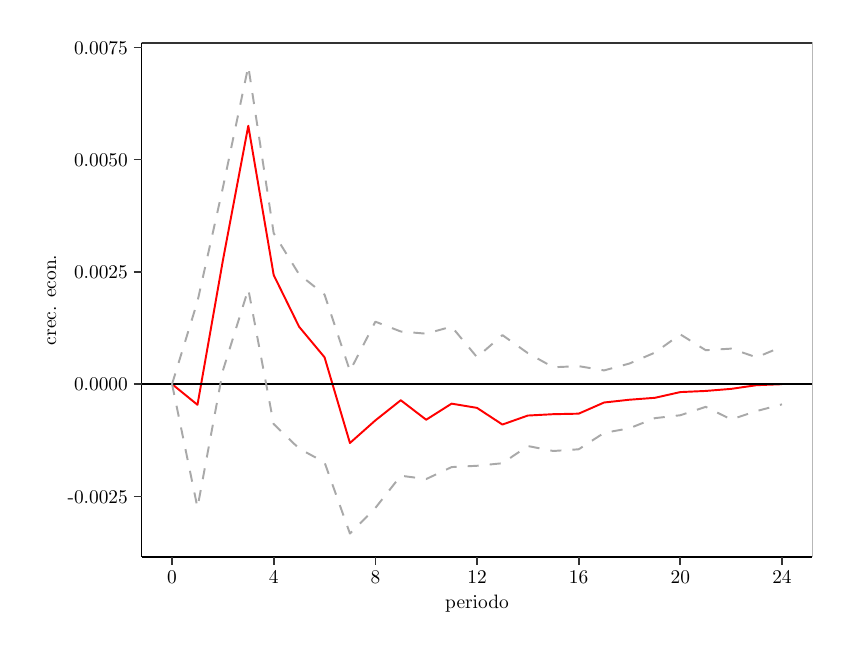
\begin{tikzpicture}[x=1pt,y=1pt]
\definecolor{fillColor}{RGB}{255,255,255}
\path[use as bounding box,fill=fillColor,fill opacity=0.00] (0,0) rectangle (289.08,216.81);
\begin{scope}
\path[clip] (  0.00,  0.00) rectangle (289.08,216.81);
\definecolor{drawColor}{RGB}{255,255,255}
\definecolor{fillColor}{RGB}{255,255,255}

\path[draw=drawColor,line width= 0.6pt,line join=round,line cap=round,fill=fillColor] (  0.00,  0.00) rectangle (289.08,216.81);
\end{scope}
\begin{scope}
\path[clip] ( 41.15, 25.56) rectangle (283.58,211.31);
\definecolor{drawColor}{RGB}{255,0,0}

\path[draw=drawColor,line width= 0.7pt,line join=round] ( 52.17, 88.02) --
	( 61.36, 80.53) --
	( 70.54,132.70) --
	( 79.72,181.36) --
	( 88.90,127.42) --
	( 98.09,108.72) --
	(107.27, 97.71) --
	(116.45, 66.73) --
	(125.64, 74.90) --
	(134.82, 82.18) --
	(144.00, 75.14) --
	(153.18, 80.95) --
	(162.37, 79.42) --
	(171.55, 73.40) --
	(180.73, 76.65) --
	(189.92, 77.14) --
	(199.10, 77.33) --
	(208.28, 81.36) --
	(217.46, 82.37) --
	(226.65, 83.06) --
	(235.83, 85.13) --
	(245.01, 85.54) --
	(254.20, 86.29) --
	(263.38, 87.62) --
	(272.56, 87.98);
\definecolor{drawColor}{RGB}{0,0,0}

\path[draw=drawColor,line width= 0.6pt,line join=round] ( 41.15, 88.02) -- (283.58, 88.02);
\definecolor{drawColor}{RGB}{169,169,169}

\path[draw=drawColor,line width= 0.7pt,dash pattern=on 4pt off 4pt ,line join=round] ( 52.17, 88.02) --
	( 61.36,117.90) --
	( 70.54,159.01) --
	( 79.72,202.87) --
	( 88.90,142.53) --
	( 98.09,127.66) --
	(107.27,120.35) --
	(116.45, 92.76) --
	(125.64,110.57) --
	(134.82,107.02) --
	(144.00,106.23) --
	(153.18,108.79) --
	(162.37, 97.73) --
	(171.55,105.72) --
	(180.73, 99.20) --
	(189.92, 94.10) --
	(199.10, 94.50) --
	(208.28, 92.96) --
	(217.46, 95.45) --
	(226.65, 99.39) --
	(235.83,105.98) --
	(245.01,100.26) --
	(254.20,100.83) --
	(263.38, 97.68) --
	(272.56,101.52);

\path[draw=drawColor,line width= 0.7pt,dash pattern=on 4pt off 4pt ,line join=round] ( 52.17, 88.02) --
	( 61.36, 43.39) --
	( 70.54, 92.90) --
	( 79.72,122.34) --
	( 88.90, 73.56) --
	( 98.09, 64.71) --
	(107.27, 59.75) --
	(116.45, 34.01) --
	(125.64, 43.26) --
	(134.82, 54.91) --
	(144.00, 53.70) --
	(153.18, 58.03) --
	(162.37, 58.50) --
	(171.55, 59.42) --
	(180.73, 65.64) --
	(189.92, 63.84) --
	(199.10, 64.46) --
	(208.28, 70.39) --
	(217.46, 72.05) --
	(226.65, 75.71) --
	(235.83, 76.76) --
	(245.01, 79.79) --
	(254.20, 75.24) --
	(263.38, 78.27) --
	(272.56, 80.69);
\definecolor{drawColor}{gray}{0.20}

\path[draw=drawColor,line width= 0.6pt,line join=round,line cap=round] ( 41.15, 25.56) rectangle (283.58,211.31);
\end{scope}
\begin{scope}
\path[clip] (  0.00,  0.00) rectangle (289.08,216.81);
\definecolor{drawColor}{RGB}{0,0,0}

\path[draw=drawColor,line width= 0.6pt,line join=round] ( 41.15, 25.56) --
	( 41.15,211.31);
\end{scope}
\begin{scope}
\path[clip] (  0.00,  0.00) rectangle (289.08,216.81);
\definecolor{drawColor}{RGB}{0,0,0}

\node[text=drawColor,anchor=base east,inner sep=0pt, outer sep=0pt, scale=  0.70] at ( 36.20, 45.04) {-0.0025};

\node[text=drawColor,anchor=base east,inner sep=0pt, outer sep=0pt, scale=  0.70] at ( 36.20, 85.60) {0.0000};

\node[text=drawColor,anchor=base east,inner sep=0pt, outer sep=0pt, scale=  0.70] at ( 36.20,126.17) {0.0025};

\node[text=drawColor,anchor=base east,inner sep=0pt, outer sep=0pt, scale=  0.70] at ( 36.20,166.73) {0.0050};

\node[text=drawColor,anchor=base east,inner sep=0pt, outer sep=0pt, scale=  0.70] at ( 36.20,207.29) {0.0075};
\end{scope}
\begin{scope}
\path[clip] (  0.00,  0.00) rectangle (289.08,216.81);
\definecolor{drawColor}{gray}{0.20}

\path[draw=drawColor,line width= 0.6pt,line join=round] ( 38.40, 47.45) --
	( 41.15, 47.45);

\path[draw=drawColor,line width= 0.6pt,line join=round] ( 38.40, 88.02) --
	( 41.15, 88.02);

\path[draw=drawColor,line width= 0.6pt,line join=round] ( 38.40,128.58) --
	( 41.15,128.58);

\path[draw=drawColor,line width= 0.6pt,line join=round] ( 38.40,169.14) --
	( 41.15,169.14);

\path[draw=drawColor,line width= 0.6pt,line join=round] ( 38.40,209.70) --
	( 41.15,209.70);
\end{scope}
\begin{scope}
\path[clip] (  0.00,  0.00) rectangle (289.08,216.81);
\definecolor{drawColor}{RGB}{0,0,0}

\path[draw=drawColor,line width= 0.6pt,line join=round] ( 41.15, 25.56) --
	(283.58, 25.56);
\end{scope}
\begin{scope}
\path[clip] (  0.00,  0.00) rectangle (289.08,216.81);
\definecolor{drawColor}{gray}{0.20}

\path[draw=drawColor,line width= 0.6pt,line join=round] ( 52.17, 22.81) --
	( 52.17, 25.56);

\path[draw=drawColor,line width= 0.6pt,line join=round] ( 88.90, 22.81) --
	( 88.90, 25.56);

\path[draw=drawColor,line width= 0.6pt,line join=round] (125.64, 22.81) --
	(125.64, 25.56);

\path[draw=drawColor,line width= 0.6pt,line join=round] (162.37, 22.81) --
	(162.37, 25.56);

\path[draw=drawColor,line width= 0.6pt,line join=round] (199.10, 22.81) --
	(199.10, 25.56);

\path[draw=drawColor,line width= 0.6pt,line join=round] (235.83, 22.81) --
	(235.83, 25.56);

\path[draw=drawColor,line width= 0.6pt,line join=round] (272.56, 22.81) --
	(272.56, 25.56);
\end{scope}
\begin{scope}
\path[clip] (  0.00,  0.00) rectangle (289.08,216.81);
\definecolor{drawColor}{RGB}{0,0,0}

\node[text=drawColor,anchor=base,inner sep=0pt, outer sep=0pt, scale=  0.70] at ( 52.17, 15.79) {0};

\node[text=drawColor,anchor=base,inner sep=0pt, outer sep=0pt, scale=  0.70] at ( 88.90, 15.79) {4};

\node[text=drawColor,anchor=base,inner sep=0pt, outer sep=0pt, scale=  0.70] at (125.64, 15.79) {8};

\node[text=drawColor,anchor=base,inner sep=0pt, outer sep=0pt, scale=  0.70] at (162.37, 15.79) {12};

\node[text=drawColor,anchor=base,inner sep=0pt, outer sep=0pt, scale=  0.70] at (199.10, 15.79) {16};

\node[text=drawColor,anchor=base,inner sep=0pt, outer sep=0pt, scale=  0.70] at (235.83, 15.79) {20};

\node[text=drawColor,anchor=base,inner sep=0pt, outer sep=0pt, scale=  0.70] at (272.56, 15.79) {24};
\end{scope}
\begin{scope}
\path[clip] (  0.00,  0.00) rectangle (289.08,216.81);
\definecolor{drawColor}{RGB}{0,0,0}

\node[text=drawColor,anchor=base,inner sep=0pt, outer sep=0pt, scale=  0.70] at (162.37,  6.86) {periodo};
\end{scope}
\begin{scope}
\path[clip] (  0.00,  0.00) rectangle (289.08,216.81);
\definecolor{drawColor}{RGB}{0,0,0}

\node[text=drawColor,rotate= 90.00,anchor=base,inner sep=0pt, outer sep=0pt, scale=  0.70] at ( 10.32,118.44) {crec. econ.};
\end{scope}
\end{tikzpicture}
